\chapter{SmartIO}\label{chapter:smartio}
SmartIO is a solution for allowing the local resources of a machine,~i.e., memory and devices, to be shared with and used by remote machines, over standard \gls{pcie}.
%
Our solution works for \emph{all} standard \gls{pcie} devices and their Linux device drivers, no special adaptation is needed in either hardware or software to make this sharing possible.
%
SmartIO is fully distributed and avoids dedicated servers.
%
All machines in the cluster~network may contribute their own local resources and access remote resources.
%
Furthermore, as remote devices and memory resources are accessed over native \gls{pcie}, they can be shared and used by remote machines with very low latency and extremely low computing overhead.
%
Whether devices are actually local or remote becomes irrelevant to the user, as SmartIO eliminates this distinction, with regard to both functionality and performance.
%
In other words, SmartIO is a flexible and efficient solution for scaling out and using more hardware resources than there are available in a single machine.


\section{Underlying idea}\label{sec:idea}
\begin{figure}
    \centering
    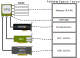
\includegraphics{bus-enumeration}
    \caption[Devices are mapped to the same address space as the \glsfmtshort{cpu} and system memory]
    {Device memory regions (\glsxtrshortpl{bar}) are mapped to the same address space as \glsxtrshort{cpu} and system memory, allowing
    the \gls{cpu} to read from and write to device memory the same way it would access \glsxtrshort{ram}. Devices can similarly use \gls{dma} to read from and write to \glsxtrshort{ram}.}
    \label{fig:bus-enumeration}
\end{figure}
The defining feature of \gls{pcie}~\cite{spec:PCIe} is that devices are mapped into the same address space as the \gls{cpu} and \gls{ram}, as seen in \cref{fig:bus-enumeration}.
%
This allows a \gls{cpu} to read from and write to device memory in the same manner it would access \gls{ram}, also known as \gls{mmio}.
%
Likewise, devices capable of \gls{dma} may read from and write to \gls{ram} directly.
%
\Gls{pcie} also uses \gls{msi}, allowing devices to raise interrupts by writing to an address reserved by the \gls{cpu} instead of requiring dedicated interrupt lines.



This address space mapping occurs when a system enumerates the \gls{pcie} bus and accesses the \gls{cfgspace} of each device.
%
A \gls{cfgspace} contains a description of the capabilities of a device, such as its memory regions.
%
The system will reserve a memory address range for each of these device memory regions, and by writing the start address of these regions to the device's \glspl{bar}, a device is made aware of the address space mapping.
%
Therefore, the term ``\gls{bar}'' is used interchangeably for a region of device memory.
%
Addresses reserved by the system for interrupts are also written to the device's \gls{cfgspace}.
%
For more details on \gls{pcie}, particularly how memory transactions are routed, please refer to \paperref{tocs:pcie,cc:pcie}.



\begin{figure}
    \centering
    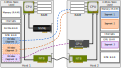
\includegraphics[width=.99\textwidth]{ntb-example}
    \caption[Two computer systems connected using \glsfmtshortpl{ntb}, and the \glsfmtshortpl{ntb} translate between the two different address domains]
    {Two computer systems connected together using \glspl{ntb} and external cables. Host~1 has mapped \glspl{segment} of Host~2's memory through its local \gls{ntb}, providing Host~1 with ``windows'' into the remote system's address space. The \glspl{ntb} translate addresses between the two independent address spaces.}
    \label{fig:ntb-example}
\end{figure}



As depicted in \cref{fig:ntb-example}, it is possible to connect computer systems with different address spaces together over \gls{pcie} by using \glspl{ntb}.
%
\Glspl{ntb} can be embedded as a \gls{cpu} feature~\cite{whitepaper:Sullivan2010,url:LinuxNTB-AMD}, but are more commonly implemented in \gls{pcie} switch chips~\cite{whitepaper:PLX,pex8733}.
%
By using such \gls{ntb}-capable switch chips to implement peripheral devices, independent computer systems can connect with plug-in host adapter cards and external cables.
%
To the system, the \gls{ntb} appears as a normal \gls{pcie} device\footnote{The \gls{pcie} terminology for individual \glspl{devicefunction} is ``\glspl{ep}''. We use the terms ``device'' and ``\gls{function}'' as synonyms for a \gls{pcieep} throughout this dissertation.} with one or more \glspl{bar} that are reserved and mapped during the enumeration process.
%
However, rather than being backed by device registers or device memory, the \gls{ntb} instead forwards reads and writes to its \glspl{bar} from one side of the \gls{ntb} to the other, translating memory addresses in the process.
%
The \gls{ntb} uses a \gls{lut} for address translation, which can be configured dynamically during run-time.
%
By using different base offsets in this \gls{lut}, it is possible to configure several memory-mappings (or ``windows'') into the address space of a remote system.
%
\Cref{fig:ntb-example} illustrates how arbitrary memory addresses on the remote system can be mapped, allowing the local \gls{cpu} to access remote memory as if it was local device memory.
%
Although address translation between the different address spaces is very fast since the \gls{lut} is implemented in \gls{ntb} hardware, the number of \gls{ntb} windows is limited by the maximum number of table entries.
%
More details on how \glspl{ntb} work can be found in \paperref{tocs:pcie-ntb}.



Since device memory on a remote system is part of the same address space as system memory, we can use an \gls{ntb} to map memory of a remote device.
%
We show this in \cref{fig:ntb-example}, where Segment~3 is allocated in \gls{gpu} memory rather than system~\gls{ram}, but still mapped for the \gls{cpu} of Host~1's similarly to the other \glspl{segment}.
%
By mapping all \glspl{bar} of a remote device for a local \gls{cpu}, it would be possible to perform memory operations on the remote device, such as reading from or writing to device registers.
%
Moreover, device~\gls{dma} is not limited to reading and writing to system \gls{ram}, but can also be used to access memory on other devices in the same address space.
%
This is known as ``\gls{p2p}'' in \gls{pcie}, and provides us with an opportunity as it becomes possible for a device to read and write directly across an \gls{ntb}.
%
We can use this to map memory resources for a device, be it \gls{ram} or memory of other devices. 
%
Furthermore, because \gls{pcie} uses \gls{msi}, it is even possible to map interrupt addresses through an \gls{ntb}, as they too are mappable.




\section{Main challenges}\label{sec:challenges}
Although \glspl{ntb} provide the fundamental memory mapping capabilities that can facilitate the use of remote devices, the challenge is to avoid requiring that device drivers must be aware of remote-side address spaces.
%
As touched upon in \cref{sec:motivation}, this is desirable in order to use existing device driver implementations.
%
For a device driver running on a local~machine to be able to use a remote~device, we must make sure that the driver uses addresses that is mapped through both the local and remote \glspl{ntb}.
%
For instance, when the device driver attempts to access \glspl{devicebar}, we must make sure that the driver uses memory addresses that are mapped through the \gls{cpu}-side \gls{ntb} without the driver or device being aware of this.
%
Conversely, when the device driver attempts to initiate \gls{dma} transfers or configures an interrupt vector address, we must find a way to transparently inject memory addresses that are mapped through the remote, or device-side, \gls{ntb}.



One possibility is to use virtualization to mitigate the complexity of managing different address spaces.
%
The fact that devices are on the other side of an \gls{ntb} could be hidden for device drivers by distributing devices to \gls{vm} \glspl{guest} instead of physical \lgls{host}{host~machines}, for example with \gls{passthrough}.
%
However, while \gls{passthrough} allows devices to be used by \glspl{vmguest} directly, \emph{requiring} that compute tasks run in \glspl{vm} will limit the generality of a solution.
%
Virtualization is not necessarily appropriate in all circumstances, as \gls{cpu} cycles are spent on \lgls{host}{hosting} the virtualized environment, thus adding additional system load.
%
Instead, a more general mechanism is needed for abstracting away the complexity of dealing with a remote-side address space.
%
This mechanism must support abstracting remote address spaces for \glspl{vm} and bare-metal machines alike.



\Gls{dma} is particularly challenging in this context.
%
A device driver running on the \gls{hostmachine} may assume that any local memory address can be reached by the device, but as explained in \cref{sec:idea}, the \gls{ntb} only provide \emph{windows} into a remote address space.
%
It is generally not possible to predict in advance which memory addresses a device driver may use, yet memory must be mapped through the \gls{ntb} before the driver, unaware that the device is remote, initiates \gls{dma} transfers.
%
Deferring the action of mapping memory through the \gls{ntb} until a device driver initiates \gls{dma}, or some other time when the specific addresses of \gls{dma} buffers and \gls{vm} memory can be known, is not viable;
%
synchronizing with the remote system at this time will introduce communication overhead in the performance-critical path.
%
The naive solution is to map the entire system memory for the device, but this workaround requires the \gls{ntb}~\glspl{bar} to be at least \emph{as large} as the size of \gls{ram}.
%
This does not scale very well, as it would effectively limit the number of machines the cluster can support.
%
Each new machine using a device would increase the device-side \gls{ntb} memory requirements by its entire \gls{ram} size.
%
Moreover, as the number of maps supported by an \gls{ntb} is also limited (by the size of its \gls{lut}), it is crucial to conserve memory maps wherever possible.
%
We must find a way to prepare memory-maps through the \gls{ntb} in advance of use, in order to avoid adding communication latency in the critical path, and without requiring that the entire memory is mapped for the device.



The challenge of \gls{dma} transfers is compounded for \gls{vmpassthrough}.
%
\Gls{passthrough} is possible by using the \gls{iommu} to create a virtual \gls{io} address space for a device that corresponds to the virtual address space of the \gls{vm}~\cite{url:LinuxVFIO,url:LinuxIOMMU,Muli2006}, also known as the ``\gls{guestphys} address space''.
%
For \gls{passthrough} of a local device, this makes it possible for the device driver running in the \gls{vmguest} to use any (virtualized) memory address when initiating \gls{dma} transfers.
%
In our case, however, the driver must use addresses that are mapped through the \gls{ntb} in order for a remote device to reach local \gls{hostphys} memory.
%
In order to support \gls{passthrough}, we must devise a method for mapping the physical memory backing the \gls{vmemulator} through the \gls{ntb}, using device-side \gls{io} addresses that mirrors the \gls{guestphys} address space.



The published papers provide further details on the challenges facing our solution as part of the description of the implementation of the different components of SmartIO.
%
Particularly \paperref{tocs:lending,tocs:mdev,tocs:nvme} provide a more in-depth explanation of what the main challenges are, and they also explain how SmartIO tackle them.
%
A discussion of additional considerations is given in \paperref{tocs:disc}.



\section{Implementation}\label{sec:implementation}
In our framework, computer systems act as \emph{``\glspl{borrower}''} and \emph{``\glspl{lender}''}.
%
A \gls{lender} is a computer system that registers one or more of its internal \gls{pcie} devices with SmartIO, allowing these devices to be distributed to and used by remote machines.
%
A \gls{borrower} is a system that is currently using such a device. 
%
While a device only has one \gls{lender}, namely the computer system where it is physically installed, there can be several \glspl{borrower} using it simultaneously.
%
SmartIO also makes it possible for a system to act as both \gls{lender} and \gls{borrower} at the same time, lending out its own local devices and simultaneously borrowing remote devices from other machines.



Basing our framework on standard \gls{pcie} is a deliberate design choice.
%
Not only does this allow commodity devices to be operated remotely by standard device drivers over native \gls{pcie}, but this design also means that the implementation complexity of SmartIO lies entirely in software.
%
In fact, SmartIO can be implemented for existing computer systems that are connected using \glspl{ntb} in any network topology, regardless of whether the \glspl{ntb} are switch chips soldered onto a motherboard or implemented as plug-in adapter cards.



Unlike other solutions for distributed \gls{io}, SmartIO combines traditional \gls{io} with distributed shared-memory functionality in a seamless manner.
%
Sharing is supported at multiple abstraction levels:
%
devices may be distributed to physical \glspl{hostmachine} and to \glspl{vm} alike.
%
Individual \lgls{function}{device functions} of \lgls{function}{multi-function} devices may be distributed to different machines in the network, or to the same machine should it require multiple resources.
%
SmartIO also provides software facilities for \gls{disaggregating} devices and memory resources, allowing device drivers to be implemented as part of distributed cluster applications or other \gls{userspace} applications. 
%
This makes it possible for several machines to simultaneously share a single \lgls{function}{device~(function)}.
%
It is even possible to \emph{combine} the sharing methods of SmartIO. 
%
For example, we can \gls{disaggregate} the device memory of a remote \gls{gpu} using the \gls{apiext} while it is being borrowed through \gls{dl}, or we can share \glspl{vf} of an \gls{sriov} \gls{nic} with both physical \glspl{hostmachine} and \glspl{vm}.


\begin{figure}
    \centering
    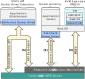
\includegraphics{software-architecture}
    \caption[Three different sharing methods are made possible by our framework. The SmartIO driver abstracts away the physical location of a remote resource]
    {The software architecture of SmartIO. Three different sharing methods are made possible by our framework: \textbf{(1)}~\gls{dl}, \textbf{(2)}~\gls{mdev}, and \textbf{(3)}~using the \gls{sisciapiext}. The SmartIO driver, shown as layer \textbf{(B)}, abstracts away the physical location of remote resources, for both the shared device and software using the device.}
    \label{fig:architecture}
\end{figure}


In this section we address the challenges of \cref{sec:challenges}, and give a bottom-up summary of the implementation of SmartIO.
%
\cref{fig:architecture} illustrates the different components of our framework, and how they fit together.
%
The implementation is described in full in the published papers, with \cref{paper:tocs} providing a detailed description of the entire solution as a whole.



\subsection{Low-level NTB driver}\label{sec:ntb-driver}
SmartIO is implemented on top of the \gls{ntb} interconnection solution from Dolphin.
%
The low-level \gls{ntb} driver, illustrated as layer \textbf{(A)} in \cref{fig:architecture}, provides the fundamental \gls{pcie} networking infrastructure and memory mapping functionality which SmartIO builds on.
%
Individual systems may contribute parts, or \emph{\glspl{segment}}, of their local memory to a distributed, shared memory space. 
%
\Glspl{memorysegment} in remote machines may be mapped into the local address space of a system by using the \gls{ntb}, as explained in \cref{sec:idea}.
%
Moreover, \gls{userspace} applications may use the \gls{sisciapi} to interact with the \gls{ntb} driver to manage \glspl{memorysegment} and implement shared-memory communication.



\subsection{SmartIO driver}\label{sec:smartio-driver}
The SmartIO driver, shown as layer \textbf{(B)} in \cref{fig:architecture}, runs on all machines in the cluster.
%
It acts as an abstraction layer, providing a logical decoupling of devices and which physical machines they are installed in (\glspl{lender}).
%
Neither devices nor software need to consider where resources physically reside, since SmartIO resolves this on behalf of both devices and a machines using them (\glspl{borrower}).
%
By providing this abstraction, the SmartIO driver is the first step towards \gls{dl}, \gls{mdev}, and the \gls{sisciapiext}, presented in \cref{sec:lending,sec:mdev,sec:api} respectively.


Devices registered with SmartIO are assigned a unique identifier which allows machines to refer to a device without needing to specify the \gls{lendermachine}.
%
Internally, the SmartIO driver keeps track of devices and \glspl{lender}, and uses this device identifier to look up machines, devices, and which \gls{ntb} to use.
%
The SmartIO driver is also responsible for making \glspl{devicebar} available as \glspl{sharedsegment}, making it possible for \glspl{borrowermachine} to memory map remote device memory into their local address space (\gls{mmio}).



Most important is the SmartIO driver's responsibility of mapping \glspl{memorysegment} \textbf{on behalf of a device} and returning the \gls{io} addresses to these maps, \textbf{as seen by the device}.
%
The SmartIO driver works out the physical locations of devices and \glspl{memorysegment},~i.e., which machines they reside in and which \glspl{ntb} a device must use in order to reach a \gls{segment}.
%
Note that a \gls{segment} can reside in memory of the machine using the device~(the \gls{borrower}), in memory of the machine where the device is installed~(the \gls{lender}), or a different cluster machine altogether.
%
A segment can even be allocated in device memory of another device, as the SmartIO driver can assist in mapping device \glspl{bar} and enabling \gls{p2p} between devices.
%
\Glspl{borrower} are not required to know anything about the \emph{device-side} \gls{io} addresses returned by our SmartIO driver, other than the fact that they resolve to the same address space as the device.
%
This allows both a \gls{borrower} and the device to remain agnostic about the underlying, physical \gls{pcie} topology, as they can rely on the SmartIO driver to resolve paths in the cluster network and map resources through the appropriate \glspl{ntb}.



The SmartIO driver solves the challenge of managing multiple address spaces, as described in \cref{sec:challenges}.
%
For example, a \gls{borrower} can request a \gls{memorysegment} in a different machine is mapped so that the device may use \gls{dma} to it.
%
Our SmartIO driver will look up which machine the \gls{memorysegment} is in, look up the \gls{lendermachine} and which (device-side) \gls{ntb} it must use, configure the \gls{ntb}, map the \gls{memorysegment} for the device, and return the device-side \gls{io} address of this map back to the \gls{borrower}.
%
The \gls{borrower} can then use this \gls{io} address when interacting with the device in order to initiate the \gls{dma} transfer, and the device is able to reach the \gls{memorysegment} through the lender's \gls{ntb}.
%
\Glspl{borrower} do not need to be aware of the internal \gls{io} address space layout of a \gls{lender}.
%
As it happens, \glspl{borrower} do not even need to know which physical machine the \gls{lender} is.



With the abstraction the SmartIO driver provides, our framework is able to facilitate the sharing and use of remote resources (both memory and devices) as described in \cref{sec:lending,sec:mdev,sec:api}.
%
More details on how SmartIO resolves the paths between devices and other memory resources that must be mapped (for devices) are given in the papers, particularly in \paperref{tocs}.
%
However, please note that the SmartIO driver is not mentioned explicitly by name in the papers, as it is the unifying base for the sharing methods.
%
Instead, the description of its functionality is interleaved with the implementation details of these methods.



\subsection{Device Lending}\label{sec:lending}
\Gls{dl}, illustrated as arrow \textbf{(1)} in \cref{fig:architecture}, makes it possible to share and distribute devices to remote \glspl{hostmachine}.
%
The devices become part of the system they are shared with, allowing application software, device drivers, and even the \gls{os} to use them as if they were locally installed.
%
While \gls{dl} only allows individual \glspl{devicefunction} to be distributed to a single machine at the time, it is nevertheless highly suitable in the case where a device has a complex or proprietary device driver as no modifications to existing software is required.



\begin{figure}
    \centering
    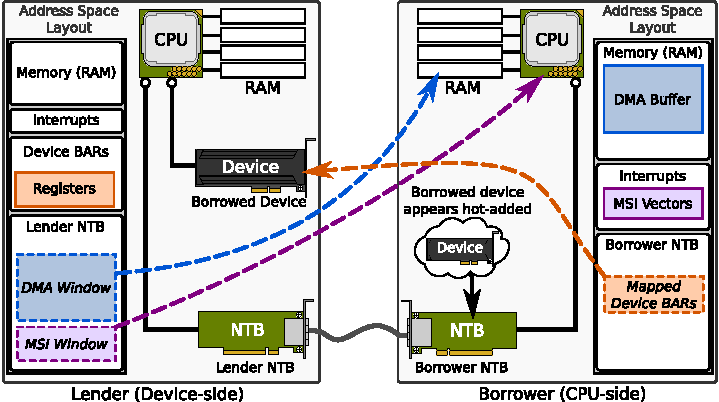
\includegraphics[width=.99\textwidth]{device-lending}
    \caption
    [The memory regions of a remote device is mapped for the \glsfmtshort{cpu} on the borrower, so that it can read and write to device registers. Local resources are mapped for the device, so that it may use \glsfmtshort{dma} and trigger interrupts. \Glsentrytext{dl} inserts a \glsentrytext{shadowdev} into the local device tree using these mappings, making remote device access transparent to both \glsfmtshort{cpu} and device.]
    {The memory regions of a remote device is mapped for the \gls{cpu} on the borrower, so that it can read and write to device registers. Local resources are mapped for the device, so that it may use \gls{dma} and trigger interrupts. \Gls{dl} inserts a \gls{shadowdev} into the local device tree using these mappings, making remote device access transparent to both \gls{cpu} and device.}
    \label{fig:device-lending}
\end{figure}

As mentioned in \cref{sec:idea}, it is possible to map the device memory regions, or \glspl{bar}, of a remote device through an \gls{ntb}.
%
Using the \gls{ntb}, a local \gls{cpu} can perform memory operations on a remote device, such as reading from and writing to device registers.
%
Conversely, local resources, such as \gls{ram} and interrupt addresses, can in turn be mapped for the remote device itself. 
%
This allows the remote device to use \gls{dma} through the \gls{ntb} and trigger interrupt routines on the local \gls{cpu}.
%
The SmartIO driver, as explained in \cref{sec:smartio-driver}, eliminates the complexity of managing multiple address spaces: a user may rely on the SmartIO driver to map resources through the appropriate \glspl{ntb} and provide \gls{io} addresses corresponding to a device's address space.
%
However, as pointed out in \cref{sec:challenges}, we still need to make sure that device drivers use this functionality without requiring that they be re-written. 
%
More precisely, we need a mechanism for \emph{transparently} injecting resolved \gls{io} addresses, without the devices or their drivers being aware of this.



\Gls{dl} solves this by inserting a ``\gls{shadowdev}'' into the local \gls{pcie} device tree on the \gls{borrower}, as depicted in \cref{fig:device-lending}. 
%
The \gls{shadowdev} makes it appear as if the remote device has been \gls{hotadded} to the local system, and provides us with a mechanism for intercepting interactions with the device by the \gls{os} and any device drivers. 
%
We make sure that a device driver attempting to memory map the device's \glspl{bar} use addresses that map through the \gls{ntb}, without the driver being aware that the device is actually remote.
%
Similarly, when the device driver configures interrupts, we are able to intercept this and inject an address that map through the \gls{lender}'s \gls{ntb}, again without the driver being aware.



The \gls{shadowdev} also provides us with the means to detect when a device driver is allocating \gls{dma} buffers and making memory available for \gls{dma} transfers.
%
Unlike \glspl{devicebar} and \gls{msi} addresses, memory addresses for \gls{dma} buffers are not known in advance, as mentioned in \cref{sec:challenges}.
%
Mapping \glspl{bar} and interrupts is a one-time operation.
%
The pages used for \gls{dma} memory buffers, however, may be scattered in physical memory.
%
A driver may even initiate several transfers to different parts of memory altogether.
%
Mapping individual memory pages through the \gls{lender}'s \gls{ntb} would not only exhaust the number of available entries in its \gls{lut}, but communicating with the \gls{lendermachine} in order to map these pages dynamically would introduce communication latency in the critical performance path.



\begin{figure}
    \centering
    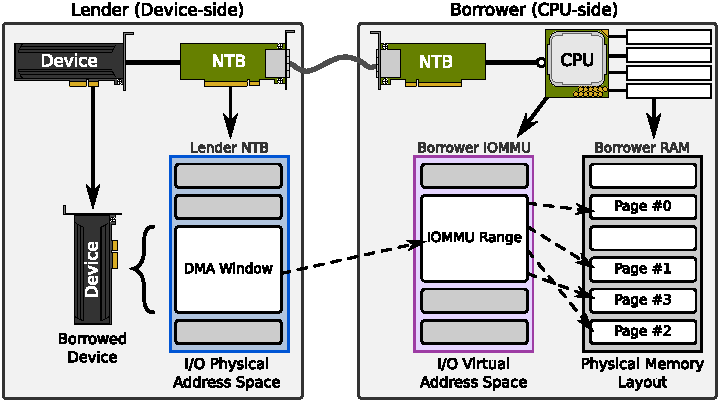
\includegraphics[width=.99\textwidth]{dma-window}
    \caption[The borrower's \glsfmtshort{iommu} is used to create a single continuous memory range that may be mapped through the lender's \glsfmtshort{ntb} in advance. Adding and removing memory pages from the local \glsfmtshort{iommu} domain is inexpensive compared to actively communicating with the remote lender~machine]
    {The \gls{borrower}'s \gls{iommu} is used to create a single continuous memory range that may be mapped through the \gls{lender}'s \gls{ntb} in advance. Adding and removing memory pages from the local \gls{iommu} domain is inexpensive compared to actively communicating with the remote \gls{lendermachine}.}
    \label{fig:dma-window}
\end{figure}




To solve this, \gls{dl} relies on the \gls{iommu} on the \gls{borrower}, as depicted in \cref{fig:dma-window}.
%
We can prepare a continuous memory address range \emph{in advance} using the \gls{borrower}'s \gls{iommu}.
%
This range can be mapped through the \gls{lender}'s \gls{ntb} with a single map, or ``\gls{dmawindow}'', even before any device drivers are using the device.
%
When a device driver, at a later point, allocates \gls{dma} buffers, we can simply add these addresses to the \gls{iommu} range.
%
This way, we can avoid making any assumptions about the memory used by a device driver.
%
Additionally, since this is an entirely local operation (on the \gls{borrower}), communication with the remote \gls{lendermachine} is avoided.
%
All address translations between the different address domains are done in \gls{ntb} and \gls{iommu} hardware, ensuring that this solution is able to achieve native \gls{pcie} performance in the data path.



A more technical description of the implementation of \gls{dl} can be found in \paperref{tocs:lending}, including details about the \gls{shadowdev} and \glspl{cfgcycle}.
%
\paperref{tocs:lending-p2p,cc:p2p} explain how \gls{dl} is able to support \gls{p2p} \gls{dma} between multiple borrowed devices, even when they reside in different \glspl{lendermachine}.
%
In addition, \paperref{tocs:lending-dma,tocs:disc-devs} explain how we can use the \emph{\gls{lender}'s} \gls{iommu} to remap \glspl{dmawindow} from high to low memory addresses for devices with addressing limitations.



\subsection{MDEV}\label{sec:mdev}
Our \gls{mdev} implementation, shown as arrow \textbf{(2)} in \cref{fig:architecture}, enables the Linux~\gls{kvm} to \emph{\lgls{passthrough}{pass through}} borrowed devices to \glspl{vm}.
%
This \gls{passthrough} allows software running in a \gls{vmguest} to use the physical device directly, without compromising the memory isolation provided by the virtualization.
%
Whereas \gls{dl} is only supported for machines running Linux, \gls{mdev} makes it possible to share devices with \emph{any} \gls{guestos} (running in the \gls{vm}).
%
Using \gls{mdev}, devices are no longer tightly coupled with the \glspl{hostmachine} they are installed in, allowing \glspl{vm} to be distributed across different \glspl{host} in the cluster while benefiting from the bare-metal performance of direct access to physical hardware.


\begin{figure}
    \centering
    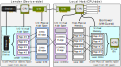
\includegraphics[width=.99\textwidth]{mdev-dma}
    \caption
    [The \glsfmtshortpl{iommu} on both sides of the \glsfmtshort{ntb} must be used in order to pass through a remote device to a local \glsfmtshort{vm}. The borrower's \glsfmtshort{iommu} is used to provide continuous memory ranges for scattered \glsfmtshort{vm} memory, while the lenders's \glsfmtshort{iommu} is used to mirror the guest-physical layout for the device]
    {The \glspl{iommu} on both sides of the \gls{ntb} must be used in order to \lgls{passthrough}{pass through} a remote device to a local \gls{vm}. The \gls{borrower}'s \gls{iommu} is used to provide continuous memory ranges for scattered \gls{vm} memory, while the \gls{lender}'s \gls{iommu} is used to mirror the \gls{guestphys} layout for the device.}
    \label{fig:mdev-dma}
\end{figure}


Our \gls{mdev} sharing method is implemented using the mediated device driver \gls{paravirtualization} interface~\cite{url:LinuxMDEV}.
%
Comparable to the \gls{shadowdev} used by \gls{dl}~(\cref{sec:lending}), this interface makes it possible to \gls{trap}~(handle) certain operations, such as \glspl{cfgcycle} and device resets, and to set the memory addresses of the device's \glspl{bar}.
%
However, unlike \gls{dl}, we do not have any means of controlling which \gls{io} addresses a device driver should use when initiating \gls{dma} transfers.
%
In \gls{dl}, we create a single, continuous \gls{iommu} range ahead of time, and map it through the \gls{lender}'s \gls{ntb}. 
%
We are able to detect when a device driver is preparing \gls{dma} buffers through the \gls{shadowdev}, and can inject the prepared device-side \gls{io} address of our \gls{dmawindow}.
%
In contrast, a device driver running in the \gls{vmguest} is completely isolated, leaving us without any equivalent mechanism to inject \gls{io} addresses we can control.
%
The only possible option is to make sure that the device is mapped to the same virtual address space as the \gls{vm}, as pointed out in \cref{sec:challenges}.



In order for a device to \gls{dma} to \gls{vm} memory, the \gls{hostphys} memory pages backing the emulated memory needs to be locked in physical \gls{ram}.
%
In practice, all memory allocated for a \gls{vmguest} must be mapped for the device, as a device driver or application running in the \gls{guest} may try to use any \gls{guestphys} address when interacting with the device.
%
However, as this is handled by the \gls{hypervisor} for normal \gls{passthrough} of a local device, the mediated device driver interface does not provide any notification of when this memory is allocated by a \gls{vmemulator}.
%
As such, we have no reliable method of detecting \gls{hostphys} memory that needs to be mapped. %through the \gls{ntb}.
%
To further complicate matters, we cannot rely on modifying existing \gls{emulator} software to solve this issue, as per our objectives stated in \cref{sec:problem}.
%
Nevertheless, it is possible to rely on an assumption:
%
before a device can use \gls{dma}, it must be enabled in its \gls{cfgspace}.\footnote{Enabling the ``Bus Master'' bit in the command register enables \gls{dma} for a device.}
%
Since the mediated device driver interface makes it possible to \gls{trap} \glspl{cfgcycle}, our \gls{mdev} implementation waits for \gls{dma} to be enabled.
%
By then, the \gls{emulator} has allocated all of the \gls{host}~memory it needs for the \gls{vm}, and we are able to use the \gls{hypervisor} to lock the \gls{hostphys} pages of the \gls{vm} in physical \gls{ram} and resolve their physical addresses.



With the \gls{hostphys} memory backing the \gls{vm} resolved, we can now map it for the device.
%
However, when \lgls{passthrough}{passing through} a local device, the \gls{hypervisor} places the device in a \gls{iommu} domain with \gls{io} virtual addresses that correspond to the \gls{vm}'s address layout.
%
In our case, the device resides in a \emph{different} machine,~i.e., the \gls{lender}.
%
Additionally, the \gls{hostphys} memory pages used by the \gls{emulator} may be scattered throughout physical \gls{ram}.
%
Our \gls{mdev} implementation solves this by using both the \gls{iommu} on the \gls{borrower} and on the \gls{lender}, as shown in \cref{fig:mdev-dma}.
%
The \gls{borrower}'s \gls{iommu} is used to provide continuous address ranges that can be mapped through the \gls{lender}'s \gls{ntb}, or \glspl{dmawindow}.
%
The \gls{iommu} on the \gls{lender} is used to map the device to a virtual \gls{io} address space that mirrors the \gls{vmguest}'s, allowing a device driver running in the \gls{vmguest} to initiate \gls{dma} transfers using \gls{guestphys} addresses.


\paperref{tocs:mdev} provides more information about the \gls{mdev} implementation, including a more detailed description of the mediated device driver interface and the functionality it provides. 
%
In the same section, we also explain a workaround for interrupts, by relaying them from the \gls{lender} to the \gls{borrower}.
%
A method of probing the \gls{kvm} using well-defined starting addresses for high and low memory is outlined, in order to pinpoint the \gls{guestphys} memory layout and conserving \gls{ntb} maps.
%
Finally, we also discuss some security implications of our \gls{passthrough} approach in \paperref{tocs:disc-security}.



\subsection{API extension}\label{sec:api}
As mentioned in \cref{sec:ntb-driver}, a \gls{userspace} application may memory-map \glspl{sharedsegment} into its own local address space using the \gls{sisciapi}.
%
Application processes running on different machines may read and write to remote memory, as if it was reading or writing to local \gls{ram}.
%
Our \gls{apiext}, depicted as arrow \textbf{(3)} in \cref{fig:architecture}, adds device-oriented programming semantics and device driver support functionality to this shared-memory \gls{api}.
%
This extension makes the core SmartIO capabilities, as described in \cref{sec:smartio-driver}, available through the same shared-memory \gls{api} used to write cluster applications.



The \glspl{bar} of a device is exported as \glspl{sharedsegment} that may be mapped by the application, providing access to device registers and other device memory (\gls{mmio}).
%
Several application processes running on different machines may even access such memory mapped \glspl{bar} at the same time.
%
Similarly, \glspl{memorysegment} can be mapped for a device (as \glspl{dmawindow}), allowing devices to use native \gls{dma} to access \gls{sharedsegment} directly.
%
These \glspl{segment} can reside in local \gls{ram} of the \gls{lender}, the \gls{borrower}, or a different cluster machine entirely.
%
\Glspl{segment} can even be allocated in device memory of \emph{other} devices.
%
SmartIO dynamically resolves the location of \glspl{segment} and devices in the cluster network, and can set up and tear down the necessary \gls{ntb} maps for the respective machines.
%
The \gls{apiext} also provides functionality for allocating \glspl{segment} associated with a device, and using access pattern hints in order for SmartIO to determine which machine it should allocate memory in.



By allowing device drivers to be implemented as part of the application software, we make it possible for devices and device operation to become part of the same shared global address space as distributed shared-memory applications.
%
Thus, device drivers can be implemented in a way that fully utilize the capabilities of \gls{pcie} networks.
%
For instance, applications may stream data to several destinations in a single operation, replicating data across several machines by relying on \gls{multicasting} support in the \gls{pcie} hardware.\footnote{\gls{pciemulticasting} is defined in the \gls{pcie} specification~\cite{spec:PCIe}}
%
A programmer can exploit memory locality to optimize data flow through the network without needing to be aware of the actual network topology, by specifying memory access pattern hints and allowing SmartIO to decide where \glspl{segment} should be allocated.
%
It is even possible to combine the \gls{apiext} with the other sharing methods of SmartIO, allowing \gls{disaggregation} of \emph{borrowed} resources.
%
An example of this is would be a machine using \gls{dl} to borrow a remote \gls{gpu} capable of \gls{gpudirect}~\cite{url:GPUDirect,url:Rosetti2014}, allowing the device to be operated by the native driver, and then using the \gls{apiext} to export \gls{gpu} memory as a \gls{sharedsegment}.
%
Application processes on other machines can then memory map this (remote) device memory \gls{segment}, allowing them to read and write directly to it as if it was local memory.



Since the \gls{apiext} is built on the underlying SmartIO driver, software can be written in a way that does not need to consider whether resources are local or remote.
%
However, using the \gls{apiext} requires the implementation of new device driver software.
%
Implementing a driver from scratch may not be a viable option in many cases, as it typically entails a considerable engineering effort.
%
After all, the strength of \gls{dl} and the \gls{mdev} implementation is precisely that they do not require any modifications to existing device driver software.
%
Even so, being able to integrate device drivers into the cluster application itself may potentially be very useful for some application domains.
%
The possibilities created by the \gls{apiext} are perhaps best exemplified by our proof-of-concept \gls{nvme} driver, described in \cref{sec:nvme-driver}.
%
This driver shows how a non-\gls{sriov} \gls{nvme} can be \gls{disaggregated} in software and shared by several machines, as well as how we can use the \gls{apiext} for \gls{disaggregating} memory resources.
%
A more specific description of the functionality added to \gls{sisci} by our \gls{apiext} can be found in \paperref{tocs:api}.



\subsection{Proof-of-concept NVMe driver}\label{sec:nvme-driver}
Most device drivers are written in a way that assumes exclusive control over the device.
%
In most cases, a device can only be distributed to a single \gls{borrowermachine} at the time, preventing others from using it while it is used.
%
Some devices implement \gls{sriov}~\cite{spec:SRIOV}, making a single physical device to appear as multiple (virtual) device functions, or \glspl{vf}.
%
Using \gls{dl} or our \gls{mdev} implementation, it is possible to distribute such \glspl{vf} to \glspl{borrower}.
%
However, due to the complexity of supporting virtualization in hardware, \gls{sriov} is not widely available, especially not for commodity devices.
%
By facilitating \gls{disaggregation} in \emph{software} instead, our \gls{sisciapiext}~(\cref{sec:api}) makes it possible for several application processes running on different machines to share the same device (\gls{function}).
%
As a demonstration of this software-enabled \gls{disaggregation}, we have implemented an \gls{nvme} driver as a \gls{userspace} \gls{sisci} application.
%
\Glspl{nvme} are highly parallel by design, and the interaction between driver software and \gls{nvme} hardware is standardized~\cite{spec:NVMe}, making it possible to implement a general device driver for them.


\begin{figure}
    \centering
    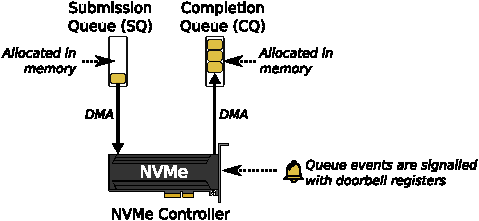
\includegraphics{nvme}
    \caption
    [\Glsfmtshortpl{nvme} support parallel and asynchronous operation by using independent queues. Queues are hosted in memory, and an \glsfmtshort{nvme} uses \glsfmtshort{dma} to fetch commands]
    {\Glspl{nvme} support parallel and asynchronous operation by using independent queues for submitting \gls{io} commands and receiving completions. Queues are hosted in memory, and an \gls{nvme} uses \gls{dma} to fetch commands and post completions.}
    \label{fig:nvme}
\end{figure}



\Cref{fig:nvme} shows how \glspl{nvme} support asynchronous operation by using a system of paired command \glspl{sq} and \glspl{cq}.
%
Both types of queues are data structures that are allocated in memory by discretion of the driver, and may be placed in \emph{any} memory location.
%
The driver submits \gls{io} commands, such as reading or writing $N$ blocks from storage, to an \gls{sq}.
%
The \gls{nvme} will use \gls{dma} to fetch commands from the \gls{sq}, and once a command is carried out, the \gls{nvme} posts the command completion status to the associated \gls{cq} (also using \gls{dma}) containing the status of the command.
%
``\Glspl{db}'' on the \gls{nvme} device are used to signal when new commands should be fetched, and each queue has its own \gls{db}.
%
Furthermore, as \emph{multiple} of these queue pairs can be created, \glspl{nvme} avoid any contention in the command submission and completion paths.
%
An example of this is a multi-core \gls{cpu} that assigns an \gls{sq} and an associated \gls{cq} per \gls{cpu} core, allowing each core to operate the \gls{nvme} independent of others.


\begin{figure}
    \centering
    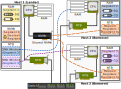
\includegraphics[width=.99\textwidth]{nvme-driver}
    \caption
    [Several machines can operate the same \glsfmtshort{nvme} simultaneously by distributing queues]
    {Several machines can share and operate the same \gls{nvme} simultaneously by distributing queues. Using the \gls{sisciapiext}, \glspl{memorysegment} with the queues' data structures can be mapped for the device, and \glspl{db} can be memory mapped for application processes.}
    \label{fig:nvme-driver}
\end{figure}


As shown in \cref{fig:nvme-driver}, our own driver implementation works by taking this one step further, allowing \glspl{cpu} in different machines to operate an \gls{nvme} simultaneously using their own queue pairs.
%
Each machine allocates a \gls{memorysegment} where it sets up the queues' data structures, and uses the \gls{apiext} to map these segments for the device as \glspl{dmawindow}.
%
This allows the \gls{nvme} to read \gls{sq} memory and write to \gls{cq} memory the same way it would access local memory, using native \gls{dma}.
%
Likewise, as \glspl{devicebar} are automatically exported by SmartIO as \glspl{segment}, all machines can memory map \glspl{db} for their respective queues.
%
Since queues are completely parallel, all the machines can submit \gls{io} commands and receive completions entirely independent of each other, once the queues are configured.
%
Note that all machines are able to operate the \gls{nvme} at the same time, including the \gls{lender}.
%
The software is the same regardless of which machine it runs on, as SmartIO keeps track of where the \glspl{segment} and the device reside.


\begin{figure}
    \centering
    \begin{subfigure}{\linewidth}
        \centering
        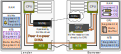
\includegraphics[width=.99\textwidth]{nvme-local-gpu}
        \caption{Storing from and loading into the memory of a \gls{gpu} residing in the \gls{borrower}.}
        \label{fig:nvme-local-gpu}
    \end{subfigure}
    \par\vspace{5mm}
    \begin{subfigure}{\linewidth}
        \centering
        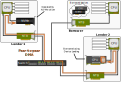
\includegraphics[width=.99\textwidth]{nvme-remote-gpu}
        \caption{Storing from and loading into the memory of a borrowed (remote) \gls{gpu}.}
        \label{fig:nvme-remote-gpu}
    \end{subfigure}
    \caption
    [Our proof-of-concept \glsfmtshort{nvme} driver is able to map \glsfmtshort{gpu} memory for an \glsfmtshort{nvme} using the SmartIO \glsfmttext{apiext}, making it possible to load and store data directly from \glsfmtshort{gpu} memory]
    {By relying on \gls{gpudirect} to expose \gls{gpu} memory through the \gls{gpu}'s \glspl{bar}, our proof-of-concept \gls{nvme} driver is able to map \gls{gpu} memory for an \gls{nvme} using the SmartIO \gls{apiext}. This makes it possible to load and store \gls{gpu} data directly, without unnecessarily copying it via \gls{ram}.}
    \label{fig:nvme-gpu}
\end{figure}


As mentioned in \cref{sec:api}, while using \gls{apiext} requires developing a new device driver, such as our proof-of-concept \gls{nvme} driver, the benefit is that device operation can become part of the cluster application itself.
%
Because SmartIO abstracts away the location of devices and \glspl{memorysegment}, the complexity of developing such distributed drivers is somewhat alleviated as software can be written in a way that does not need to consider whether resources are local or remote.
%
Any memory resource can be mapped for the device, regardless of its location in the cluster.
%
An implementation can exploit this in order to optimize the movement of data through the network---without needing to consider the actual \gls{pcie} topology.
%
It is even possible to combine the use of the \gls{apiext} with the other sharing methods of SmartIO.
%
Our \gls{nvme} driver demonstrates some of the possibilities created by the \gls{apiext}: 
%
\begin{description}
    \item[Remote \gls{gpu} access] (\cref{fig:nvme-gpu}):
        %
        Many \gls{gpu}-accelerated applications, such as big~data and machine~learning tasks, require access to data on a storage device.
        %
        Traditionally, loading data from a storage device and into \gls{gpu} memory involves first reading data to system memory, and then copy it onto the \gls{gpu}.
        %
        Likewise, storing the result of a \gls{gpu} computation involves copying it out of the \gls{gpu} to system memory, and then writing it to storage.
        %
        Since datasets used in typical big~data and machine~learning tasks can be as large as hundreds of terrabytes, \gls{gpu} applications become bounded by transfers between storage and \gls{gpu}.
        %
        To overcome this, some \glspl{gpu} support \gls{p2pdma}, making it possible to load data directly into \gls{gpu} memory and avoid unnecessary copies via system memory~\cite{Bergman2019,url:Thompson2019}.
        %
        For Nvidia \glspl{gpu}, this functionality is supported through the \gls{gpudirect}~\gls{api}~\cite{url:GPUDirect}, which makes on-board \gls{gpu} memory accessible through the \gls{gpu}'s \glspl{bar}.
        %
        As explained in \cref{sec:smartio-driver}, SmartIO automatically exports \glspl{devicebar} as \glspl{memorysegment}, which can be mapped for a device using the \gls{apiext}.
        %
        Our proof-of-concept \gls{nvme} driver use this to enable an \gls{nvme} to read and write directly to the memory of both local \glspl{gpu} and \emph{borrowed} \glspl{gpu} (using \gls{dl}), as seen in \cref{fig:nvme-local-gpu,fig:nvme-remote-gpu} respectively.
        %
        Note that the \gls{gpu} is operated by the native \gls{gpu} driver in both scenarios, but we still use the \gls{apiext} to disaggregate its device memory.

    \item[Memory locality optimizations] (\cref{fig:nvme-queues}):
        \begin{figure}
            \centering
            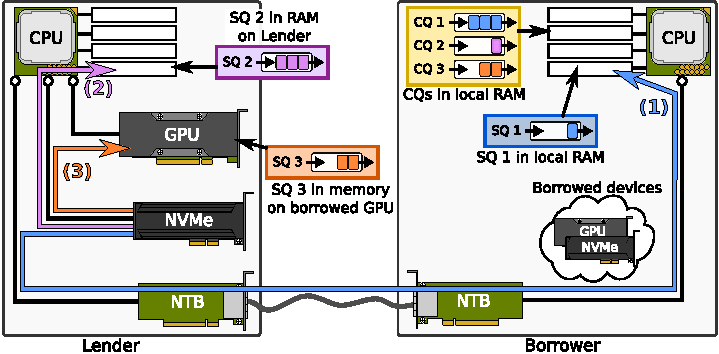
\includegraphics{nvme-queues}
            \caption
            [By using access pattern hinting, it is possible to consider memory locality without requiring the driver implementation to be aware of the underlying \glsfmtshort{pcie} topology]
            {Our \gls{nvme} driver implementation relies on SmartIO to decide where \glspl{segment} containing queues should be allocated. By using access pattern hinting, it is possible to consider memory locality without requiring the driver implementation to be aware of the underlying \gls{pcie} topology.}
            \label{fig:nvme-queues}
        \end{figure}
        %
        In \gls{pcie}, the latency of transactions are affected by the number of switch chips they need to traverse.
        %
        Particularly memory reads are affected; the longer the path between a device and the memory it reads from, the higher the latency becomes, as \gls{pcie} transactions have to travel further.
        %
        As described in \cref{sec:api}, a programmer can rely on the \gls{apiext} to decide where \glspl{segment} should be allocated, based on memory access pattern hinting.
        %
        In the case of our \gls{nvme} driver, we can use this functionality when creating \glspl{segment} for queue memory, as illustrated in \cref{fig:nvme-queues}.
        %
        By specifying that the \gls{segment} containing \glspl{cq} will be written to by the \gls{nvme}, and read by the \gls{borrower}'s \gls{cpu}, SmartIO will decide to allocate the \gls{segment} in memory closer to the \gls{cpu},~i.e., in the \gls{borrower}'s local \gls{ram}.
        %
        Similarly, a segment with an \gls{sq} can be allocated in the \gls{lender}'s \gls{ram} by specifying that the \gls{nvme} will read from it and the \gls{cpu} will only write to it, shown as SQ1 in \cref{fig:nvme-queues}.
        %
        It is even possible to use memory of \emph{another device} for \glspl{sq}.
        %
        By mapping \gls{gpu} memory for the device, as explained above, it is possible to allocate the \gls{sq} on a borrowed \gls{gpu} that is close to the \gls{nvme}, depicted as SQ2 in \cref{fig:nvme-queues}.

    \item[Initiating \gls{io} directly from the \gls{gpu}] (\cref{fig:nvme-gpu-offloading}):
\begin{figure}
    \centering
    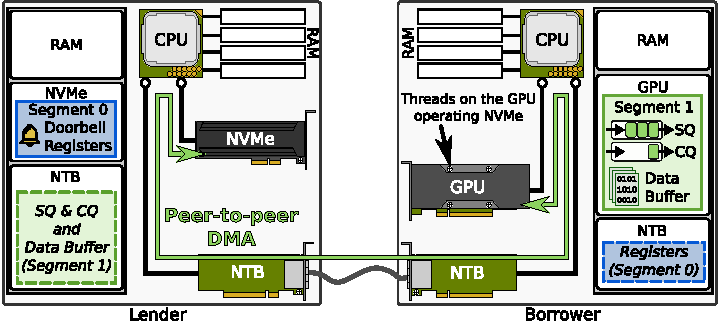
\includegraphics{nvme-gpu-offloading}
    \caption
    [Our \glsfmtshort{nvme} driver can run on a \glsfmtshort{gpu} independently of the \glsfmtshort{cpu}]
    {Our \gls{nvme} driver can also run on a \gls{gpu}. \Gls{gpu} threads can submit \gls{io} commands and wait for completions independent of the \gls{cpu}.}
    \label{fig:nvme-gpu-offloading}
\end{figure}
        %
        Similarly to how \gls{gpu} memory can be mapped for an \gls{nvme} using SmartIO, it is also possible to map \glspl{db} for the \gls{gpu}.
        %
        The logic for submitting \gls{io} commands to an \gls{sq} and polling an \gls{cq} for completions is also supported for \gls{cuda} applications in our \gls{nvme} driver implementation.
        %
        As such, \textbf{our \gls{nvme} driver may run on a \gls{gpu}}, allowing \gls{gpu} threads to read from and write to storage directly without any involvement of the \gls{cpu}.
        %
        The performance of \gls{cuda} applications that work with large data sets, such as machine~learning workloads, can be increased, as loading and storing data at various points in the computation no longer requires synchronization with software running on the \gls{cpu}.
        

\end{description}


A more technical description of the implementation of the proof-of-concept \gls{nvme} driver can be found in \paperref{tocs:nvme}.
%
Here, we describe how the driver is split into a manager and a client component, with the manager being responsible for resetting the device and assigning queues to clients.
%
We also explain how our implementation can support multi-path fail-over, and how \gls{pciemulticasting} can be used to replicate data loaded from storage across machines in a single operation.
%
More details on how it is possible to run the \gls{nvme} driver as part of a \gls{cuda} application can also be found here.



\section{Performance measurements}\label{sec:eval}
Our SmartIO framework makes it possible for machines to use remote \gls{pcie} devices in a manner that is indistinguishable from using local resources, both functionally and performance wise.
%
Since remote devices can be used without requiring any modifications to either application software or device drivers, it is possible to use standard benchmarking tools and existing application to evaluate SmartIO.
%
A complete evaluation of SmartIO in the form of a comprehensive collection of performance tests can be found in the published papers, ranging from microbenchmarks aimed at evaluating a specific component to realistic, large-scale workloads:
%
\begin{itemize}

    \item In \paperref{nossdav:eval}, the initial \gls{dl} implementation is evaluated using an Nvidia \gls{gpu}, comparing the performance of \gls{dma} transfers of a borrowed (remote) \gls{gpu} to a local \gls{gpu}.
        %
        We also compare the performance of native \gls{dma} to a \gls{pcie}-based \gls{rdma} implementation, to demonstrate the performance benefit of native \gls{dma} transfers to remote memory.

    \item A \gls{gpu}-based video processing workload is presented in \paperref{mmsys}. \Gls{dl} is used to scale up the number of available \glspl{gpu} for the workload, in order to meet a real-time deadline.
        %
        To demonstrate \gls{dl} and \gls{mdev} being used for real-world applications, we also evaluate the run-time performance of a machine~learning workload using borrowed \glspl{gpu} and an borrowed \gls{nvme} in \paperref{cc:eval-ml}.

    \item We perform \gls{p2p} experiments with \glspl{gpu} in several network topologies in \paperref{srmpds:eval}, evaluating the effect longer \gls{pcie} paths have on \gls{dma} performance. These tests are extended in \paperref{cc:eval} with additional network topologies and test scenarios.
        %
        We also evaluate the \gls{mdev} implementation using a \lgls{passthrough}{passed-through} \gls{nvme}, and show the impact \glspl{iommu} have on on \gls{dma} transfers. 

    \item An exhaustive performance evaluation of the final implementation of SmartIO is presented in \paperref{tocs:eval}, evaluating all parts of the implementation from multiple angles.
        %
        This evaluation also use a wide variety of different Linux distributions, benchmarking software, and different \gls{pcie} devices, in order to demonstrate that our SmartIO framework is not limited to a specific Linux version or any specific device, but works for a wide variety of different software versions and devices.
        %
        We prove that, when conditions are similar, our SmartIO sharing methods \textbf{do not add any performance overhead} compared to using local resources.
        %
        Additionally, \paperref{tocs:eval-nvme} also present several experiments using our our proof-of-concept \gls{nvme} driver.
        %
        Several capabilities made possible through the \gls{sisciapiext} are demonstrated, such as an experiment with 30~cluster~nodes sharing a single-function \gls{nvme} simultaneously, how data stored on the \gls{nvme} can be \lgls{multicasting}{multicasted} an replicated across 60~nodes in a single operation, as well as interoperability with both local and remote \glspl{gpu}.
\end{itemize}



In this section, we present the performance measurements for three selected benchmarks, showing that our SmartIO framework is able to facilitate the use of remote \gls{pcie} devices with the same performance as if these devices were locally installed.
%
The first two tests are comparison tests, where we compare the performance of an \gls{io}-heavy workload running on a local system using a local \gls{io} resource, to the same workload running on a remote machine using the same resource borrowed through \gls{dl}.
%
With all conditions being the same, from the software to the devices being used, a comparison between the measurements for both the local run and remote run should reveal any performance overhead introduced by SmartIO.
%
The third test is intended to demonstrate memory optimization functionality in our proof-of-concept \gls{nvme} driver enabled by the \gls{apiext}, by making it possible to allocate \glspl{sq} in different kinds of memory.



All three tests involve two Intel~Xeon machines, and PXH830 \gls{ntb} adapter cards from Dolphin~\cite{pxh830}.
%
Additional \gls{pcie} network topologies are evaluated in the published papers, including larger clusters.
%
In order to create a \gls{pcie} topology that is similar for local and remote test runs, we have used a BP-457-ATX \gls{pcie} expansion chassis from One~Stop~Systems.
%
By using an expansion chassis, there are the same number of \gls{pcie} switch chips (or ``hops'') in the path between the \gls{cpu} and the device in both the local and remote scenarios.%
\footnote{We show how longer \gls{pcie} paths affects \gls{dma} performance in \paperref{cc:eval-native-p2p,tocs:eval-lending-path,tocs:eval-lending-p2p-2L}.}
%
Moreover, the switch chips are the same  Broadcom~PEX8733~\cite{pex8733} chips used in the implementation of the Dolphin \gls{ntb} adapter cards.
%
Standard and unmodified benchmarking software are used for our tests, and for first two \gls{dl} tests we have used standard device drivers.



\subsection{Device Lending: latency comparison}\label{sec:eval-lat}
\begin{figure}
    \centering
    \begin{subfigure}{\linewidth}
        \centering
        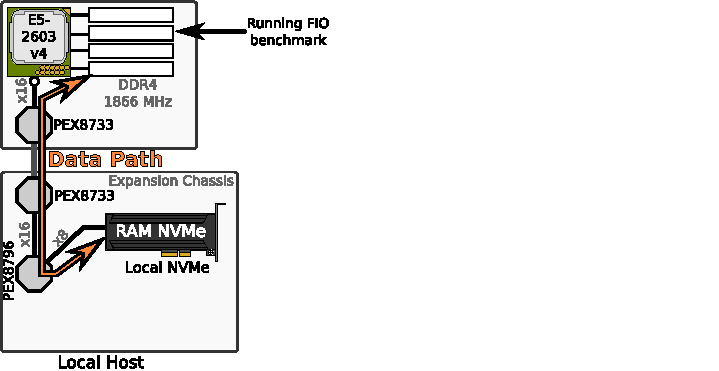
\includegraphics[width=.99\textwidth]{lending-experiments-local-nvme}
        \caption{\textbf{Local Baseline}: an \glsxtrshort{nvme} in an expansion chassis attached to the local \glsxtrshort{pcie} bus.}
        \label{fig:eval-lending-nvme-local}
    \end{subfigure}
    \par\vspace{10mm}
    \begin{subfigure}{\linewidth}
        \centering
        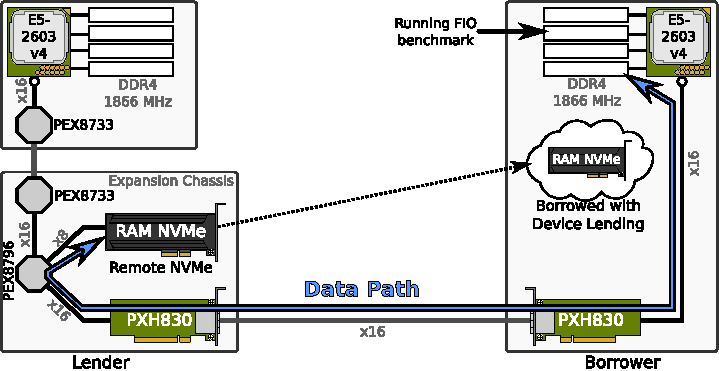
\includegraphics[width=.99\textwidth]{lending-experiments-remote-nvme}
        \caption{\textbf{Device Lending}: a borrowed \glsxtrshort{nvme}, appearing local to the remote system.}
        \label{fig:eval-lending-nvme-remote}
    \end{subfigure}
    \par\vspace{5mm}
    \caption[Hardware configuration for the two scenarios in our latency comparison experiment. By using an expansion chassis, the \glsfmtshort{nvme} is the same number of ``hops'' away from the \glsfmtshort{cpu} using the device for both scenarios]
    {Hardware configuration for the two scenarios in our latency comparison experiment. By using an expansion chassis, the \glsxtrshort{nvme} is the same number of ``hops'' away from the \glsxtrshort{cpu} using the device for both the Local~Baseline and \gls{dl} scenarios. The only difference is whether the switch chips are configured in transparent mode or \glsxtrshort{ntb} mode. The data path is illustrated for both scenarios.}
    \label{fig:eval-lending-nvme-topo}
\end{figure}



Using the \gls{dl} sharing method, machines may use remote resources in the same way it would use local resources.
%
Consequently, it possible to run a workload locally first, establishing a ``baseline'' for expected performance measurements.
%
The same workload can then be repeated on a remote system using borrowed devices, allowing us to compare performance measurements to this ``local baseline''.
%
Any difference in the measured performance will reveal whether or not \gls{dl} adds any performance overhead compared to local access.



We have used the \gls{fio}~\cite{url:fio} to create a synthetic storage workload and measure the latency of reading from disk.
%
\Gls{fio} is a widely used \gls{userspace} application for benchmarking the performance of storage devices, such as \glspl{nvme}.
%
However, as the purpose of the test is \emph{not} to benchmark the \gls{nvme} itself, but rather any potential overhead of our \gls{dl} sharing method, we used a prototype \gls{ram} disk with an \gls{nvme} controller from PMC-Sierra.
%
This is to avoid any effects caused by prefetching and caching, that modern \glspl{ssd} are capable of.




\begin{figure}
    \centering
    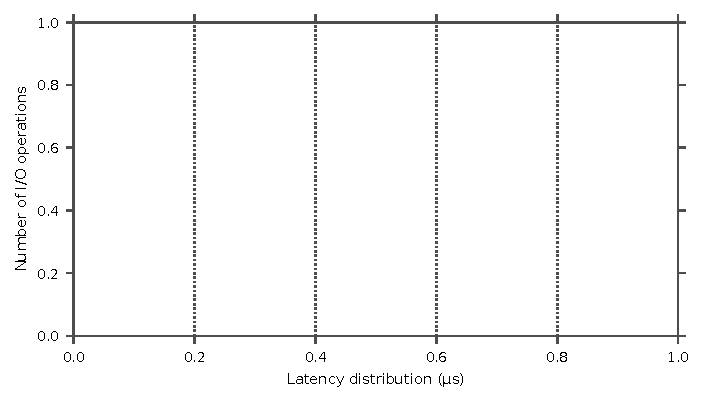
\includegraphics[width=.99\textwidth]{lending-nvme}
    \caption
    [Histogram of the latency distributions for reads from storage for both the Local~Baseline and Device~Lending scenarios. The distributions overlap, demonstrating that our implementation does not add any overhead in the critical \glsfmtshort{io} path]
    {Histogram of the latency distributions for reads from storage for both the Local~Baseline and \gls{dl} scenarios. The distribution for both scenarios overlap, demonstrating that our implementation does not add any overhead in the critical \glsxtrshort{io} path.}
    \label{fig:eval-lending-nvme-results}
\end{figure}
%
\Cref{fig:eval-lending-nvme-topo} shows the topologies for our test scenarios:
\begin{description}
    \item[Local Baseline] (shown in \cref{fig:eval-lending-nvme-local}):%
        An external expansion chassis with the \gls{nvme} installed, connected to a local machine. 
        %
        The expansion chassis is connected upstream using One Stop System's HIB68-x16 target adapter cards and external \gls{pcie} cables. 
        %
        These adapters use the same Broadcom~PEX8733 \gls{pcie} switch chip used in the Dolphin PXH830 \gls{ntb} adapters.
        %
        The \gls{iommu} is disabled, in order to make the configuration comparable to the \gls{dl} scenario described below.
        
    \item[\Gls{dl}] (shown in \cref{fig:eval-lending-nvme-remote}):
        %
        Two machines connected together in a back-to-back topology, using Dolphin~PXH830 adapter cards and external \gls{pcie} cables.
        %
        The remote \gls{nvme} is borrowed using \gls{dl}.
        %
        The \gls{iommu} is disabled on both the \gls{lender} and \gls{borrower}.
        %
        The same expansion chassis configuration as in the local baseline scenario is used, and since the \gls{lender}'s \gls{iommu} is disabled, \gls{pcie} transationcs are routed peer-to-peer as illustrated in the figure.
\end{description}



In both scenarios, the machines run CentOS~7 with a 3.10 kernel, and version~3.7 of \gls{fio} (as available from the CentOS~7 software repositories).
%
Additionally, the standard in-kernel \gls{nvme} driver is used in both scenarios.
%
We configured \gls{fio} to perform 8192 reads per run, and ran \gls{fio} 80~times per scenario and concatenated the results.
%
Each read is a page-sized block~(4~kB) at a random offset.



\Cref{fig:eval-lending-nvme-results} shows the latency distribution of read operations for both a local \gls{nvme}~(Local~Baseline) and when accessing it remotely using \gls{dl}.
%
Each data point is the latency for a full 4~kB read operation.
%
We see that the two distributions overlap, proving that there is no difference in performance for local and remote.
%
A more in-depth explanation of this experiment can be found in \paperref{tocs:eval-lending-lat}.



\subsection{Device Lending: DMA throughput comparison}\label{sec:eval-bw}
\begin{figure}
    \centering
    \begin{subfigure}{\linewidth}
        \centering
        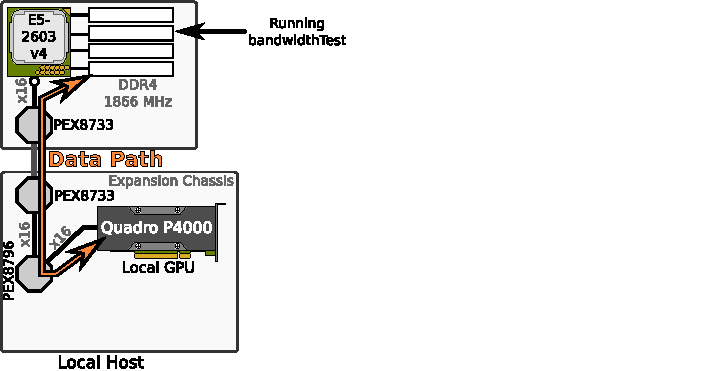
\includegraphics[width=.99\textwidth]{lending-experiments-local-gpu}
        \caption{\textbf{Local Baseline}: using a local \glsxtrshort{gpu} in an expansion chassis.}
        \label{fig:eval-lending-gpu-local}
    \end{subfigure}
    \par\vspace{10mm}
    \begin{subfigure}{\linewidth}
        \centering
        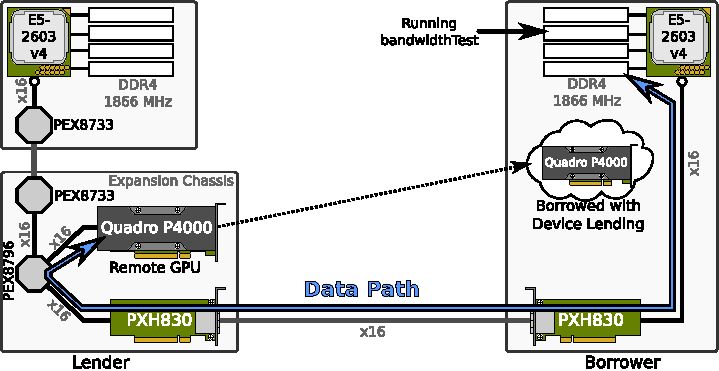
\includegraphics[width=.99\textwidth]{lending-experiments-remote-gpu}
        \caption{\textbf{Device Lending}: using a borrowed \glsxtrshort{gpu}.}
        \label{fig:eval-lending-gpu-remote}
    \end{subfigure}
    \par\vspace{5mm}
    \caption
    {Hardware configuration for the two scenarios in our \glsxtrshort{dma} throughput comparison experiment. Similar to the}
    \label{fig:eval-lending-gpu-topo}
\end{figure}


\begin{figure}
    \centering
    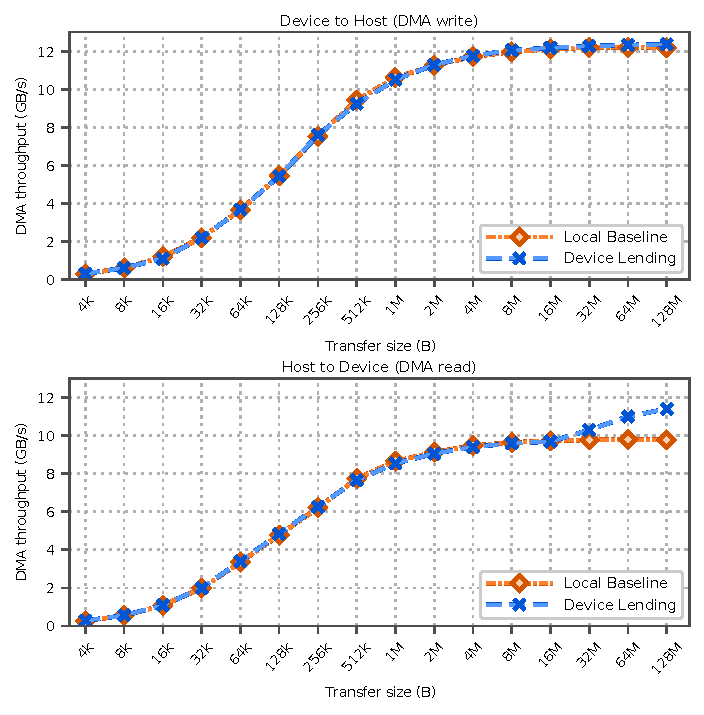
\includegraphics[width=.99\textwidth]{lending-gpu}
    \caption{test}
\end{figure}


\subsection{Proof-of-concept NVMe driver: SQ experiment}
\begin{figure}
    \centering
    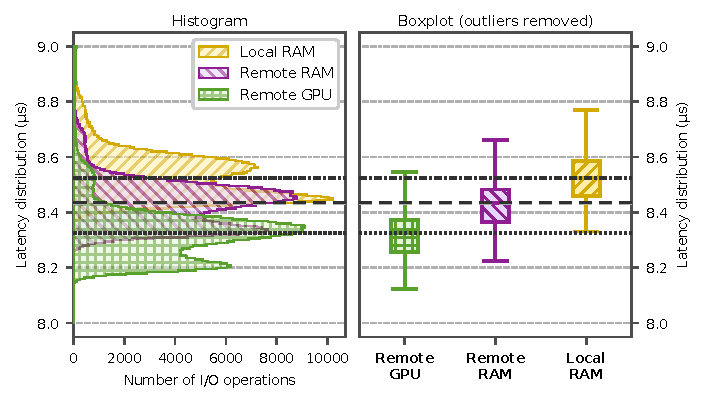
\includegraphics[width=.99\textwidth]{nvme-sq}
    \caption{test}
\end{figure}




\section{Related work}\label{sec:rw}
Sharing resources efficiently among networked machines is a wide-ranging topic that span several research areas.
%
In fact, each individual component of our solution could potentially be discussed at great length on their own, in order to place them in proper context.
%
However, at its core, SmartIO is a framework for machines in a \gls{pcie} network to share their internal devices and memory resources.
%
In this section, we attempt to give a condensed overview of related work we consider the most relevant.
%
A more detailed presentation of related work can be found in \paperref{tocs:rw}.
%
Background for the ideas behind our proof-of-concept \gls{nvme} driver is summarized in \paperref{tocs:rw-nvme}.


\subsection{Solutions not using NTBs}
State of the art within \gls{disaggregation} and resource sharing can broadly be divided into three categories:
%
\begin{itemize}
    \item So-called ``rack-scale \gls{disaggregation}'' by \textbf{logical partitioning}, where modular blade servers are connected to a backplane or a shared \gls{io} bus fabric within a data center rack.
        %
        Devices are installed in dedicated resource servers, and can be dynamically assigned to compute hosts as needed.
        %
        These solutions can be realized using interconnection technologies that are specialized for this purpose~\cite{Suzuki2016,Krishnan2006,Shrivastav2019,Katrinis2016}, but
        %
        \gls{pcie} (with additional virtualization support) is the most used alternative for commercial solutions~\cite{url:liqid,url:gigaio,Chung2018,Ravindran2008}.
        %
        We also include \gls{mriov}~\cite{spec:MRIOV} in this category, even though we are unaware of any available implementations of it.

        
        \Gls{pcie}-based solutions use switch chips with virtualization support that makes it possible to isolate devices and \glspl{cpu} by creating logical device trees for each host~\cite{Wong2011,whitepaper:Microsemi,whitepaper:IDT,Chung2018}, as illustrated in \cref{fig:partitioning}.
        %
        Some solutions even support assigning individual \glspl{vf} of an \gls{sriov}-capable device to different hosts~\cite{Chung2018}.
        %
        However, as we addressed in \cref{sec:motivation}, it is only possible to distribute resources that are directly attached to these partitionable switch chips. Sharing the \emph{internal} resources of a machine, such as its memory and local devices, is not possible.
        %
        Consequently, solutions based on switch partitioning cannot support memory-to-memory communication between hosts, nor are they able to support any memory \gls{disaggregation}.
        %
        Instead, additional \gls{disaggregation} solutions like \gls{rdma} are needed.


    \item Memory \gls{disaggregation} through \textbf{remote memory access}.
        %
        The goal of most memory \gls{disaggregation} solutions is not necessarily to make more resources available or improve resource utilization in the cluster, but rather to facilitate shared-memory communication for distributed cluster applications.
        %
        Remote memory access is most commonly implemented on top of \gls{rdma}, and made available to the application through typical parallel programming models, such as \gls{mpi}~\cite{Jiang2004} and \gls{rpc}~\cite{Lu2013}, or through more explicit abstractions~\cite{Aguilera2018}.
        %
        Approaches for accessing remote memory in a more transparent fashion also exist, usually achieved by modifying the system page fault handler to initiate \gls{rdma} transfers so remote memory pages can be ``\lgls{trap}{faulted in}''~\cite{Liang2005,Gu2017,Lim2009}.
        

        Especially \gls{mpi} protocols implemented on top of \gls{rdma} over InfiniBand appear to be widely used for distributed computing.
        %
        Many of these \gls{mpi} solutions also support \gls{gpudirect}, effectively making it possible to \gls{disaggregate} \gls{gpu} memory~\cite{Venkatesh2014,Venkatesh2017,url:Rosetti2014}.
        %
        Although \gls{rdma} enables efficient data transfer over a network through one-sided initiation and direct access to application memory, it nevertheless introduces a layer of indirection;
        %
        compared to a \gls{cpu} (or device) reading and writing to a memory-mapped location directly, latency is significantly increased by needing to initiate (and wait for) \gls{rdma} transfers.


    \item Device \gls{disaggregation} by \textbf{distributed \gls{io} over a network} using \gls{rdma}.
        %
        Examples include rCUDA for sharing \glspl{gpu} in an InfiniBand cluster~\cite{Duato2010}, and \gls{nvmeof} using \gls{rdma}~\cite{Guz2018,spec:NVMe-oF}.
        %
        Solutions for sharing \glspl{gpu}~\cite{Hou2013} and Ethernet \glspl{nic}~\cite{Tu2014} over a \gls{pcie} fabric have also been proposed, by using \gls{pcie} switch chips capable of \gls{dma} to transfer data from memory to memory in the different machines.
        

        As mentioned in \cref{sec:motivation}, \gls{rdma}-based approaches must communicate with a device driver running on the device-side system, in order to interact with the remote device.
        %
        As this is typically solved by implementing a \gls{middlewareservice} that uses an existing driver or by implementing a distributed driver, these solutions are generally specific to the (type of) device they \gls{disaggregate}.
        %
        Moreover, as illustrated in \cref{fig:direct-access}, this additional software component on the remote system inevitably leads to a performance overhead, compared to a local device driver directly interacting with a device. % on the \gls{pcie} bus.

\end{itemize}
%




With its three sharing methods, our own SmartIO framework intersects all three of these \gls{disaggregation} categories.
%
Similarly to \gls{pcie}-based rack-scale solutions, we are able to distribute devices using the \gls{dl} and \gls{mdev} sharing methods~(\cref{sec:lending,sec:mdev}), including individual \glspl{vf} of devices capable of \gls{sriov}.
%
We also have an inherent relationship with memory \gls{disaggregation} solutions, through the shared-memory functionality provided by the \gls{sisciapi} and our SmartIO extension of it~(\cref{sec:api}).
%
It is even possible to \gls{disaggregate} devices similar to \gls{rdma}-based device \gls{disaggregation}, as demonstrated by our proof-of-concept \gls{nvme} driver~(\cref{sec:nvme-driver}).
%
However, by being implemented on top of \gls{pcie} cluster networking, SmartIO is able to offer significant improvements over the other three types of \gls{disaggregation}:
%
\begin{itemize}
    \item Unlike \gls{pcie}-based rack-scale \gls{disaggregation}, where only resources attached directly to partitionable switch chips can be shared, SmartIO instead makes it possible for all machines to lend out their internal devices and borrow resources from remote machines.



    \item In contrast to \gls{rdma}-based solutions for memory \gls{disaggregation}, remote \glspl{memorysegment} can be mapped into a local software application's virtual address space directly using the \gls{sisciapi}.
        %
        Using our \gls{exttosisciapi}, we greatly extend this functionality by making it possible to map shared \glspl{memorysegment} for \emph{devices} as well.
        %
        The need to use \gls{rdma} for shared-memory communication is removed entirely, as both \glspl{cpu} and devices may instead read and write to remote memory directly.
        %
        Moreover, it becomes possible to integrate \gls{io} and device operation into the cluster application itself.



    \item Contrary to device \gls{disaggregation} using \gls{rdma}, SmartIO removes the need to interact with a remote device driver on the device-side system.
        %
        Instead, as SmartIO enables access to remote resources over native \gls{pcie} for both driver and device, devices can be operated directly by a device driver running locally on the \gls{borrower}.
        %
        As no software is needed in the performance-critical data path, SmartIO has the performance advantage of native \gls{pcie}.


    \item Using either the \gls{dl} or \gls{mdev} sharing methods, devices appear locally installed.
        %
        This makes SmartIO a more general solution compared to \gls{rdma}-based \gls{disaggregation}, in the sense that \emph{any} \gls{pcie} device may be shared and operated by existing device drivers.
        %
        However, in addition to distributing devices to both physical machines and \glspl{vm}, we also facilitate what we call ``\gls{mriov} in software'' through the \gls{sisciapiext}.
        %
        This allows non-\gls{sriov} devices to be shared with several hosts at the same time, something that is not possible with current solutions based on partitionable \gls{pcie} switch chips and requires \gls{rdma}.
        %
        SmartIO is ``the best of both worlds'', by combining the flexibility of shared-memory functionality with the ability to use remote devices as if they were locally installed.



    \item \Gls{disaggregation} of device memory is made simpler by SmartIO.
        %
        Because SmartIO abstracts away the physical \gls{pcie} topology, the device memory of both local and borrowed devices is trivially memory mapped by an application and for other devices using our \gls{sisciapiext}.
        %
        For example, applications that rely on \gls{gpudirect} can memory map (remote) \gls{gpu} memory directly, instead of needing to use abstractions such as \gls{mpi}.
        %
        Moreover, since it is also possible to borrow remote \glspl{gpu} using \gls{dl}, SmartIO supports \gls{cuda}'s native unified memory model~\cite{url:unified-memory} as well, allowing remote \glspl{gpu} to read and write to each other's memory as if they were installed in the same machine.
        %
        This makes application development significantly easier, as software can be written as if all resources are local.
        %
        We are not aware of any \gls{rdma}-based \gls{gpu} disaggregation solutions that are able to support this.

\end{itemize}

We present a more technically detailed comparison between specific solutions and our own SmartIO implementation in the published papers, particularly in \paperref{tocs:rw}.


\subsection{Solutions using NTBs}
Solutions that enable \gls{disaggregation} using \glspl{ntb} are particularly interesting to us, due to the similarities with our own work.
%
By using the same Broadcom~8733~\cite{pex8733} \gls{pcie} switch chips used in the Dolphin~PXH830 adapter cards used in our own evaluation (\cref{sec:eval}), Shim~et~al.~\cite{Shim2018} and Lim~et~al.~\cite{Lim2019} have implemented \gls{ntb} host adapter cards and connected three machines in a cluster.
%
They have extended the OpenSHMEM \gls{api} with support for their \gls{ntb} implementation.
%
However, their focus seem to be enabling \gls{pgas}-style shared memory functionality for high-performance computing applications, and distributing and sharing devices appears not to have been considered as part of their solution.
%
It should also be noted that the underlying memory-mapping functionality provided by their solution is very similar to functionality already existing in the \gls{sisciapi}.


The Ladon system~\cite{Tu2013} facilitates access to the same \gls{sriov} device from multiple \glspl{vmguest}.
%
Several machines and a \gls{sriov} device is connected to a top-of-rack \gls{pcie} switch with \gls{ntb}-capable ports.
%
The device and a dedicated ``management host'' is connected to the switch in \emph{transparent} mode, so that the management host may enumerate the \gls{pcie} bus and configures the device.
%
Multiple ``compute hosts'' are connected to the same switch through \emph{non-transparent} switch ports,~i.e., \glspl{ntb}.
%
The management host maps the entire memory of each compute host for the device, and assists the \gls{hypervisor} on each compute hosts in mapping \glspl{devicebar}, in order to \gls{passthrough} individual \glspl{vf} to \glspl{vm} running on the compute hosts.
%
It is also possible to map interrupts directly into the \glspl{vmguest}~\cite{Tu2014phd,Tu2015}.



The Ladon system is very similar to our own \gls{mdev} implementation.
%
For example, the management host is comparable to our \gls{lender}, and the compute hosts would be the equivalent to \glspl{hostmachine} that run \gls{vm} \glspl{borrower} in SmartIO.
%
However, Ladon and our own SmartIO framework differ in some areas:
\begin{itemize}
    \item 
        Only \gls{vmpassthrough} appears to be have been considered for the Ladon system.
        %
        SmartIO, on the other hand, supports sharing with both physical \glspl{hostmachine} and \glspl{vmguest}, through the \gls{dl} and \gls{mdev} sharing methods respectively.
        %
        Because the management host maps the \emph{entire} \gls{ram} of each compute host, it could in theory be possible to extend Ladon with support for physical machines. 
        %
        However, such an extension would likely require that device drivers are adapted to interact with the management host to set up mappings.
        %
        In contrast, our own \gls{dl} sharing method makes it possible for bare-metal hosts to use devices without requiring modifications to existing device driver software.

    \item
        Perhaps the main difference between Ladon and SmartIO is that while a single host,~i.e., the management host, owns the device in Ladon, our SmartIO system is truly distributed by supporting multiple machines acting as \glspl{lender}.
        %
        Machines may even act as both \gls{lender} and \gls{borrower} at the same time.
        %
        Moreover, in Ladon, the management host becomes a single point of failure.
        %
        Ladon has since been extended with fail-over support, allowing a back-up management host to replicate the \gls{pcie} fabric enumeration of the first host, and seamlessly take ownership of the device in case the first management host fails~\cite{Tu2018}.
        %
        However, we argue that this still does not make Ladon distributed in the same sense as our SmartIO solution.
        %
        For example, it is not possible for a compute host to use devices from \emph{different} management hosts.
        %
        In contrast, SmartIO supports scaling out and using devices from several machines across an entire cluster.

    \item
        The Ladon implementation relies on mapping the entire memory of all compute hosts for the device.
        %
        Because of this, the number of compute hosts that can be supported in the Ladon setup will be limited to a handful of hosts due to the combined \gls{bar} size requirements of the \glspl{ntb}.
        %
        This differs from our own \gls{mdev} implementation, where only the \gls{vm} memory is mapped for the device.
        %
        Additionally, should the \gls{ntb}'s \gls{bar} size become a limitation, it is possible to scale out and distribute devices over multiple lender systems.
        
\end{itemize}



Compared to other solutions implemented using \glspl{ntb}, SmartIO is a more comprehensive framework for sharing devices and memory resources:
%
our solution makes it possible to share devices to remote machines (both bare-metal \glspl{hostmachine} and \glspl{vm}), as well as and \gls{disaggregating} memory resources. 
%
Through the SmartIO abstraction layer, the hard distinction between local and remote is blurred out, making it easier to scale out and use remote resources.
%
Using SmartIO, it is even possible to combine sharing capabilities with shared-memory functionality, allowing devices to become part of the same global address space as distributed, shared-memory applications.
